\documentclass[mathserif,xcolor=table]{beamer}
\usepackage{etex}
\reserveinserts{28}
% ---------------------------------------------------------------------------
%				Packages
% ---------------------------------------------------------------------------

% texdoc <nom_package> pour avoir des infos

\usepackage[utf8]{inputenc}						% Encodage français
\usepackage[frenchb]{babel}						% Mise en forme française
\usepackage[T1]{fontenc}						% Encodage caractères français

\usepackage{fourier}							% Différents symboles et polices
\usepackage[scaled=0.875]{helvet}				% Font générale
\usepackage{courier}							% Font télétype
\renewcommand{\ttdefault}{lmtt}					% Font télétype
\usepackage{frcursive}							% Ecriture manuscrite type écolier
\usepackage{calligra}							% Ecriture manuscrite classieuse
\usepackage{verbatim}							% Commentaires

\usepackage{amsfonts,amsmath,amssymb}			% Symboles maths
\usepackage{bm}									% Symboles maths en gras \bm{}
\usepackage{amstext}							% Texte en mode math de taille adaptée
\usepackage{amsopn}								% \DeclareMathOperator
\usepackage{mathrsfs}							% Symboles maths
\usepackage{mathtools}							% Symboles maths
\usepackage{theorem}							% Mise en forme des théorèmes

\usepackage{textcomp}							% Symboles
\usepackage{pifont}								% Symboles "ding"
\usepackage{wasysym}							% Symboles (smiley et logos)
\usepackage{epsdice}							% Symboles (faces d'un dé)
\usepackage[normalem]{ulem}						% Fioritures de texte (barré, etc...)
\usepackage{cancel}								% Barrer du texte (simplifier termes)
\usepackage{fancybox}							% Boîtes

\usepackage{tabularx}							% Tableaux évolués
\usepackage{diagbox}							% Cases en diagonale
%~ \usepackage{tabls}							% Espaces dans les tableaux (conflit avec bclogo)
\usepackage{multirow}							% Fusionner les lignes d'un tableau
\usepackage[table]{xcolor}
\usepackage{enumerate}							% Enumérations personnalisées
%\usepackage{enumitem}							% Reprendre une énumération [start=n]
\usepackage{multicol}							% Environnement multicolonnes
\usepackage{fancyhdr}							% En-têtes et pieds de page
%~ \usepackage[np]{numprint}					% Mise en forme des nombres

%\usepackage[usenames, dvipsnames]{xcolor}		% Couleurs
\usepackage{graphicx}							% Insérer des images
\usepackage{pgf, tikz, tkz-tab, tkz-fct}		% Graphiques avec Tikz
\usetikzlibrary{arrows}
\usetikzlibrary{snakes}
\usepackage{alterqcm}							% QCM
\usepackage[tikz]{bclogo}						% Boites à logo

%\usepackage{titlesec}							% Mise en forme des titres de sections
\usepackage{lastpage}							% Dernière page : \pageref{LastPage}

\usepackage{ifthen}								% Programmation conditions
\usepackage{multido}							% Boucles
\usepackage{calc}								% Calculs

% ---------------------------------------------------------------------------
%				Macros simples (caractères)
% ---------------------------------------------------------------------------

\newcommand{\euro}{\eurologo{}}
\newcommand{\R}{\ensuremath{\mathbb{R}}}
\newcommand{\N}{\ensuremath{\mathbb{N}}}
\newcommand{\D}{\ensuremath{\mathbb{D}}}
\newcommand{\Z}{\ensuremath{\mathbb{Z}}}
\newcommand{\Q}{\ensuremath{\mathbb{Q}}}
\newcommand{\C}{\ensuremath{\mathbb{C}}}
\newcommand{\e}{\text{e}}
\renewcommand{\i}{\text{i}}
\newcommand{\s}{\ensuremath{\mathcal{S}}}
\newcommand{\sol}[1]{\mathcal{S}=\left\lbrace #1 \right\rbrace}
\newcommand{\ou}{\mbox{ ou }}
\newcommand{\et}{\mbox{ et }}
\newcommand{\si}{\mbox{ si }}
\newcommand{\Df}{\ensuremath{\mathcal{D}_f}}
\newcommand{\Cf}{\ensuremath{\mathcal{C}_f}}

\renewcommand{\P}{\ensuremath{\text{P}}}
\newcommand{\card}{\text{card}}
\newcommand{\E}{\text{E}}
\newcommand{\V}{\text{V}}

\newcommand{\FI}{\textbf{F.I.}}

\newcommand{\eq}{\ \Leftrightarrow\ } % ou \iff
\newcommand{\implique}{\Rightarrow}
\newcommand{\pheq}{\phantom{\eq}}
\newcommand{\egdef}{\stackrel{\textit{déf}}{=}}

\renewcommand{\ge}{\geqslant}
\renewcommand{\le}{\leqslant}
\newcommand{\supeg}{\geqslant}
\newcommand{\infeg}{\leqslant}

\newcommand{\lacco}{\left\lbrace}
\newcommand{\racco}{\right\rbrace}
\newcommand{\labs}{\left|}
\newcommand{\rabs}{\right|}

\newcommand{\inclus}{\subset}
\newcommand{\ninclus}{\not\subset}
\newcommand{\union}{\cup}
\newcommand{\inter}{\cap}

\newcommand{\non}[1]{\text{non(}#1\text{)}}

\newcommand{\dx}{~\text{d}x}
\newcommand{\dt}{~\text{d}t}

\renewcommand{\Re}{\text{Re}}
\renewcommand{\Im}{\text{Im}}
\newcommand{\conj}[1]{\overline{#1}}
\newcommand{\abs}[1]{|#1|}

\newcommand{\pinf}{+\infty}
\newcommand{\minf}{-\infty}
\newcommand{\pminf}{\pm\infty}

\newcommand{\para}{\ /\!\!/\ }

\newcommand{\comb}[2]{\text{C}_{#1}^{#2}}

\newcommand{\vect}[1]{\mathchoice
	{\overrightarrow{\displaystyle\mathstrut#1\,\,}}
	{\overrightarrow{\textstyle\mathstrut#1\,\,}}
	{\overrightarrow{\scriptstyle\mathstrut#1\,\,}}
	{\overrightarrow{\scriptscriptstyle\mathstrut#1\,\,}}}

\def\Oij{$\left(\text{O},~\vect{\imath},~\vect{\jmath}\right)$}
\def\Oijk{$\left(\text{O},~\vect{\imath},~ \vect{\jmath},~ \vect{k}\right)$}
\def\Ouv{$\left(\text{O},~\vect{u},~\vect{v}\right)$}

\definecolor{gris}{gray}{0.85}
\newcommand{\surl}[1]{\colorbox{gris}{\textbf{#1}}}

\renewcommand{\emph}{\textbf}

\newcommand{\saut}{\ \\}
\newcommand{\lignesep}{\vspace*{5pt}\hrule\vspace*{5pt}}

\newcommand{\fct}[5]{
	\begin{array}[t]{r ccl}
	{#1}\ : \ &{#2}&\longrightarrow&{#3}\\
	&{#4}&\longmapsto&{#5}
	\end{array}}

\newcommand{\encadre}[1]{\fbox{\begin{minipage}{\textwidth}
#1
\end{minipage}}}

%\newcommand{\boite}[1]{\fbox{\Huge\phantom{A}\hspace*{#1}}}
\newcommand{\boite}[1]{\fbox{\rule[-0.2cm]{0pt}{0.6cm}\hspace*{#1}}}


\newcommand{\suit}{\begin{tikzpicture}
\draw[color=white](-0.4em,0em)--(-0.25em,0em);
\draw ((-0.25em,-0.15em)--(0.07em,0.18em);
\draw (0.07em,0.18em) arc (135:0:0.25em);
\draw (0.5em,0em) arc (-180:-45:0.25em);
\draw (0.93em,-0.18em)--(1.36em,0.25em);
\draw (1.01em,0.25em)--(1.36em,0.25em)--(1.36em,-0.1em);
\draw[color=white](1.40em,0em)--(1.55em,0em);
\end{tikzpicture}}


%\newcommand{\suit}{\hookrightarrow}

% Commande programmation Casio

\newcommand{\touche}[1]{\fbox{\texttt{#1}}}

\newcommand{\toucheF}[2]{
$\underset{\text{\scriptsize F#2}}{\touche{#1}}$
}

\newcommand{\sto}{$\rightarrow$}

%\newcommand{\toucheFF}[2]{\begin{tabular}[t]{c}
%\touche{#1}\\
%{\scriptsize F#2}
%\end{tabular}}

\newcommand{\suiv}{$\vartriangleright$} % Menu suivant

\newcommand{\rl}{\begin{tikzpicture}[scale=0.7] % Retour à la ligne de la Casio
\draw[color=white] (0,0)--(0,0);
\draw [<-] (0.2em,0.2em)--(1em,0.2em)--(1em,0.8em);
\end{tikzpicture}}

\newcommand{\disp}{\begin{tikzpicture}[scale=0.7] % Triangle de la Casio
\draw[color=white] (0,0)--(0,0);
\fill (0.2em,0em)--(0.8em,0em)--(0.8em,0.8em)--(0.2em,0em);
\draw[color=white] (1em,1em)--(1em,1em);
\end{tikzpicture}}

\newcommand{\vers}{$\rightarrow$}

\newcommand{\enonce}{\textbf{Énoncé :}}
\newcommand{\solut}{\textbf{Solution :}}
\newcommand{\tq}{~,~}

\newcommand{\xmin}{x_{\text{min}}}
\newcommand{\xmax}{x_{\text{max}}}

% -------------------- Symboles : -------------------------------------------

\newcommand{\happy}{\smiley}
\newcommand{\sad}{\frownie}

\newcommand{\attention}{\danger}
\newcommand{\piege}{\bomb}
\newcommand{\interdit}{\noway}

\newcommand{\facede}[1]{\epsdice{#1}}

\newcommand{\hand}{\text{\ding{43}}}
\newcommand{\victory}{\text{\ding{44}}}

\newcommand{\trefle}{\text{\ding{168}}}
\newcommand{\carreau}{\text{\ding{169}}}
\newcommand{\coeur}{\text{\ding{170}}}
\newcommand{\pique}{\text{\ding{171}}}

\newcommand{\checkbox}{\text{\ding{114}}}
\newcommand{\checkedbox}{\text{\mbox{\ding{114}\hspace{-.7em}\raisebox{.2ex}[1ex]{\ding{51}}}}}

\newcommand{\scisors}{\ding{34}}
\newcommand{\couperici}{\scisors\dotfill\textit{\small{couper ici}}\dotfill\scisors}

% ---------------------------------------------------------------------------
% 				Environnements 
% ---------------------------------------------------------------------------

% ------------------------ Théorèmes ----------------------------------------
\newenvironment{Th}{\begin{block}{Théorème}}{\end{block}}
\newenvironment{Dem}{\begin{block}{Démonstration}}{\end{block}}
\newenvironment{DemBac}{\begin{block}{Démonstration BAC}}{\end{block}}
\newenvironment{Ex}{\begin{block}{Exemple}}{\end{block}}
\newenvironment{Rem}{\begin{block}{Remarque}}{\end{block}}
%\newenvironment{Rem}{\textbf{Remarque :}\\}{}
\newenvironment{Def}{\begin{block}{Définition}}{\end{block}}
\newenvironment{Prop}{\begin{block}{Propriété}}{\end{block}}
\newenvironment{Exo}{\begin{block}{Exercice}}{\end{block}}
\newenvironment{Algo}{\begin{block}{Algorithme}}{\end{block}}










%\theorembodyfont{\normalfont} \theoremstyle{break}
%\newtheorem{Th}{Théorème}[section]
%\newtheorem{Dem}{Démonstration}[section]
%\newtheorem{DemBac}{Démonstration (démo Bac)}[section]
%\newtheorem{Exmp}{Exemple}[section]
%\newtheorem{Rem}{Remarque}[section]
%\newtheorem{Def}{Définition}[section]
%\newtheorem{Nota}{Notations}[section]
%\newtheorem{Prop}{Propriété}[section]
%\newtheorem{Exo}{Exercice}[section]
%\newtheorem{App}{Application}[section]
%\newtheorem{Cons}{Conséquence}[section]
%\newtheorem{Ex}{Exemple}[section]
%\newtheorem{Algo}{Algorithme}[section]


%\newcommand{\Ex}{\noindent\textbf{Exemple : }}
\newcommand{\Rappel}{\noindent\textbf{Rappel : }}

% ------------------------ Python --------------------------------------------

\newcounter{cptspace}
%\newcommand{\tab}[1]{
%	\setcounter{cptspace}{#1}
%	\whiledo{\value{cptspace}>0}{
%		\hspace*{0em}\hspace*{0em}
%		\addtocounter{cptspace}{-1}}}

\newcommand{\tab}[1]{
	\setcounter{cptspace}{#1}
	\whiledo{\value{cptspace}>0}{
		\hspace*{0.25cm}
		\addtocounter{cptspace}{-1}}}

\newcommand{\prompt}{{>}{>}{>}\ }

\newenvironment{python}
	{\par\ttfamily\small\vspace{0.2cm}
	\setbox0=\hbox\bgroup
	\begin{minipage}{\textwidth}
	\vspace{0.2cm}
%	\begin{tabbing}
	}
	{\vspace{0.2cm}
%	\end{tabbing}
	\end{minipage}
	\egroup
    \fbox{\box0}
	\par\rmfamily\normalsize\vspace{0.2cm}\noindent
	}

\newenvironment{algo1}
	{\begin{center}\begin{tabular}{|>{\texttt\bgroup}l<{\egroup}|}
	\hline}
	{\hline
	\end{tabular}\end{center}
	}

%\newenvironment{python}
%	{\par\ttfamily\small\vspace{0.2cm}
%	\begin{bclogo}[couleurBord=black, arrondi = 0.1, logo={}, barre = none]{Code python :}
%%	\begin{minipage}{\textwidth}
%%	\vspace{0.2cm}
%	}
%	{%\vspace{0.2cm}
%%	\end{minipage}
%	\end{bclogo}
%	\par\rmfamily\normalsize\vspace{0.2cm}\noindent
%	}

\newcommand{\pyth}[1]{\texttt{#1}}

% -------------------------- Boites bclogo -----------------------------------
\newenvironment{warning}
	{\begin{bclogo}[couleurBord=black, arrondi = 0.1, logo = \bcattention]}%{\Large\attention}]}
	{\end{bclogo}}
	
\newenvironment{forbidden}
	{\begin{bclogo}[couleurBord=black, arrondi = 0.1, logo = \bcinterdit]}%{\Large\interdit}]}
	{\end{bclogo}}

% ---------------------------------------------------------------------------
% 				Raccoucis clavier
% ---------------------------------------------------------------------------

\newcommand{\fctsurI}[3]{
	Soit $#1$ la fonction définie sur $#3$ par $$#1(x)=#2$$}
	
\newcommand{\hp}{Hors programme de TSTI2D}

% ---------------------------------------------------------------------------
%				Macros évoluées
% ---------------------------------------------------------------------------

% ----------------- \tournerpage --------------------------------------------
% Indique de tourner la page en bas de page
%
\def\tournerpage{\vfill%
	\begin{flushright}	
		\textbf{Tourner la page }$\mathbf{\rightarrow}$
	\end{flushright}
	\newpage}


% -------------------- Numérotations des questions et puces -----------------

%\renewcommand{\theenumi}{\textbf{\arabic{enumi}}}
%\renewcommand{\labelenumi}{\textbf{\theenumi.}}
%\renewcommand{\theenumii}{\textbf{\alph{enumii}}}
%\renewcommand{\labelenumii}{\textbf{\theenumii.}}
%\renewcommand{\labelenumiii}{\textbullet}

\AtBeginDocument{\renewcommand{\labelitemi}{\textbullet}}
\AtBeginDocument{\renewcommand{\labelitemii}{\textbullet}}


% % -------------------- Réglages divers------------------------------------- 

\everymath{\displaystyle\everymath{}}		% Toutes les équations en mode \displaystyle
\DecimalMathComma							% Virgule comme séparateur décimal
\frenchspacing								% Espaces français
\setlength{\parindent}{0pt}					% Pas d'indentation de paragraphes

\colorlet{gris1}{black!20}
\colorlet{gris2}{black!30}

% ----------------------------------------------------------------------------

% =============================================================================
% 								FIN PREAMBULE
% =============================================================================



\useoutertheme[hooks]{tree}
\useinnertheme{rounded}
\usecolortheme{seahorse}
\usecolortheme{orchid}



\title[Bataille navale]{\textsc{Bataille navale}}
\subtitle{Projet de validation ISN 2016}
\author{Frédéric Muller}
\institute{Lycée Arbez Carme}
\date{}

\AtBeginSubsection[]
%\AtBeginSection[]
{
  \begin{frame}<beamer>
    \frametitle{Plan}
    \tableofcontents[currentsection,currentsubsection,    subsubsectionstyle=hide]
  \end{frame}
}

\AtBeginSection[]
{
  \begin{frame}<beamer>
    \frametitle{Plan}
    \tableofcontents[currentsection,currentsubsection,    subsubsectionstyle=hide]
  \end{frame}
}


\definecolor{fondalgo}{HTML}{E6D8FF}
\begin{document}

\begin{frame}
\titlepage
\end{frame}

\section{Les structures de données}
\subsection{Constantes de direction}
\begin{frame}{Constantes de direction}
\begin{itemize}
\item \texttt{DROITE = (1, 0)} 
\item \texttt{GAUCHE = (-1, 0)}
\item \texttt{BAS = (0, 1)}
\item \texttt{HAUT = (0, -1)}
\item \texttt{TOUTES\_DIR = (1, 1)}
\end{itemize}
\end{frame}

\subsection{Structure de la grille}
\begin{frame}{Initialisation}
Paramètres de la grille (modifiables) :
\begin{itemize}
\item \texttt{xmax, ymax} : dimensions de la grille
\item \texttt{taille\_bateaux} : liste contenant les bateaux
\end{itemize}\pause
Initialisations :
\begin{itemize}
\item \texttt{Grille.somme\_taille} : nombre total de cases à toucher (pour déterminer la fin de la partie).
\end{itemize}
\end{frame}

\begin{frame}{État de la grille}
Dictionnaire \texttt{Grille.etat} indexé par des tuple \texttt{(i, j)} de coordonnées de cases.\\ \pause
\texttt{Grille.etat[(i,j)]=}
\begin{itemize}
\item $0$ : case vide
\item $1$ : case touchée (ou contenant un bateau)
\item $-1$ : case manquée ou impossible
\end{itemize}
~\\ \pause
\texttt{Grille.vides} : liste des cases vides
\end{frame}

\begin{frame}
Méthodes de contrôle :
\begin{itemize}
\item \texttt{Grille.test\_case(self, case)} : \texttt{True} si la case est vide et dans la grille
\item \texttt{Grille.is\_touche(self, case)} : \texttt{True} si la case contient un bateau
\end{itemize}
\end{frame}


\begin{frame}{Espaces vides}
\texttt{Grille.get\_max\_space(self, case, direction, face=True)} : renvoie l'espace vide maximal dans une direction.\\
Si \texttt{face==True}, la détermination se fait dans les deux sens (espace libre total horizontal ou vertical).\\~\\ \pause
\texttt{Grille.elimine\_cases(self)} : élimine les cases vides dans lesquelles le plus petit bateau ne peut pas rentrer.
\end{frame}

%\begin{frame}[allowframebreaks]
%Si direction == TOUTES\_DIRECTIONS :\\
%\tab{1} On renvoie le maximum de get\_max\_space(case, HORIZONTAL)\\
%\tab{2} et get\_max\_space(case, VERTICAL)\\~\\
%direction[0]\sto dh\\
%direction[1]\sto dv\\
%1\sto m\\
%\framebreak
%case[0]\sto x\\
%case[1]\sto y\\
%Tant que la case (x+dh, y+dv) est vide et est dans la grille :\\
%\tab{1}m+1\sto m\\
%\tab{1}x+dh\sto x\\
%\tab{1}y+dv\sto y\\
%\framebreak
%Si face (on regarde dans l'autre sens):\\
%\tab{1}case[0]\sto x\\
%\tab{1}case[1]\sto y\\
%\tab{1}Tant que la case (x-dh, y-dv) est vide et est dans la grille :\\
%\tab{2}m+1\sto m\\
%\tab{2}x-dh\sto x\\
%\tab{2}y-dv\sto y\\~\\
%Retourner m\\
%\end{frame}

\begin{frame}{Bateaux possibles}
\texttt{Grille.get\_possibles(self)} renvoie :
\begin{itemize}
\item La liste des bateaux possibles démarrant sur chaque case (ainsi que leurs directions)\\
Par exemple : \texttt{\{(0,0):[(5,(1,0)), (5,(0,1)),...], (0,1):...\}}
\end{itemize}
\end{frame}

\begin{frame}
Par exemple sur la case (0,0), avec la case (3,0) déjà manquée :
\begin{center}
\begin{tikzpicture}[scale=0.5]
\draw (0,1)--(10,1);
\draw (-1,0)--(-1,-10);
%\draw (-1,0)--(10,0);
%\draw (-1,-1)--(10,-1);
%\draw (-1,-2)--(10,-2);
%\draw (-1,-3)--(10,-3);
\foreach \x in {0,1,...,10}{
\draw (\x,1)--(\x,-10);
\draw (-1,-\x)--(10,-\x);
}
\foreach \x in {0,1,...,9}{
\draw (\x+0.5,0.5) node{\x};
\draw (-0.5,-\x-0.5) node{\x};
}
\draw (3.5,-0.5) node{O};
\draw[fill=gray!30] (0,0) rectangle(1,-1);

\draw<1>[very thick] (0,0) rectangle (1,-5);
\draw<1>[very thick, ->] (0.5,-0.5)--(0.5,-4.5);
\draw<2>[very thick] (0,0) rectangle (1,-4);
\draw<2>[very thick, ->] (0.5,-0.5)--(0.5,-3.5);
\draw<3>[very thick] (0,0) rectangle (1,-3);
\draw<3>[very thick, ->] (0.5,-0.5)--(0.5,-2.5);
\draw<4>[very thick] (0,0) rectangle (3,-1);
\draw<4>[very thick, ->] (0.5,-0.5)--(2.5,-0.5);
\draw<5>[very thick] (0,0) rectangle (1,-2);
\draw<5>[very thick, ->] (0.5,-0.5)--(0.5,-1.5);
\draw<6>[very thick] (0,0) rectangle (2,-1);
\draw<6>[very thick, ->] (0.5,-0.5)--(1.5,-0.5);
\end{tikzpicture}

[ \only<1->{(5,(1,0))}\only<2->{ , (4,(1,0))}\only<3->{ , (3,(1,0))}\only<4->{ , (3,(0,1))}\only<5->{ , (2,(1,0))}\only<6->{ , (2,(0,1))} ]

\end{center}
\end{frame}


\begin{frame}{Bateaux possibles}
\texttt{Grille.get\_possibles(self)} renvoie également:
\begin{itemize}
\item La liste des positions (et directions) de départ possibles pour chaque bateau\\
\texttt{\{5:[((0,0), (1,0)), ((0,0), (0,1)), ((1,0), (1,0)),...], 4:...\}}
\end{itemize}
\end{frame}

\begin{frame}
Par exemple, pour le bateau de taille 5 :
\begin{center}
\begin{tikzpicture}[scale=0.5]
\draw (0,1)--(10,1);
\draw (-1,0)--(-1,-10);
%\draw (-1,0)--(10,0);
%\draw (-1,-1)--(10,-1);
%\draw (-1,-2)--(10,-2);
%\draw (-1,-3)--(10,-3);
\foreach \x in {0,1,...,10}{
\draw (\x,1)--(\x,-10);
\draw (-1,-\x)--(10,-\x);
}
\foreach \x in {0,1,...,9}{
\draw (\x+0.5,0.5) node{\x};
\draw (-0.5,-\x-0.5) node{\x};
}
\draw (3.5,-0.5) node{O};

\draw<1>[fill=gray!30] (0,0) rectangle(1,-1);
\draw<1>[very thick] (0,0) rectangle (1,-5);
\draw<1>[very thick, ->] (0.5,-0.5)--(0.5,-4.5);

\draw<2>[fill=gray!30] (1,0) rectangle(2,-1);
\draw<2>[very thick] (1,0) rectangle (2,-5);
\draw<2>[very thick, ->] (1.5,-0.5)--(1.5,-4.5);

\draw<3>[fill=gray!30] (2,0) rectangle(3,-1);
\draw<3>[very thick] (2,0) rectangle (3,-5);
\draw<3>[very thick, ->] (2.5,-0.5)--(2.5,-4.5);

\draw<4>[fill=gray!30] (4,0) rectangle(5,-1);
\draw<4>[very thick] (4,0) rectangle (5,-5);
\draw<4>[very thick, ->] (4.5,-0.5)--(4.5,-4.5);

\draw<5>[fill=gray!30] (4,0) rectangle(5,-1);
\draw<5>[very thick] (4,0) rectangle (9,-1);
\draw<5>[very thick, ->] (4.5,-0.5)--(8.5,-0.5);

\end{tikzpicture}

[ \only<1->{((0,0), (1,0))}\only<2->{ , ((1,0), (1,0))}\only<3->{ , ((2,0), (1,0))}\only<4->{ , ((4,0), (1,0))}\only<5->{ , ((4,0) ,(0,1))...} ]

\end{center}
\end{frame}

\begin{frame}
\begin{center}
etc...
\end{center}
\end{frame}

\begin{frame}{Gestion de la flotte}
Gestion de la liste \texttt{Grille.taille\_bateaux} :
\begin{itemize}
\item \texttt{Grille.get\_taille\_max(self)} et \texttt{Grille.get\_taille\_min(self)} : mise à jour respectivement de la taille maximum et la taille minimum des bateaux restant à trouver
\item \texttt{Grille.rem\_bateau(self, taille)} : supprime un bateau de la liste \texttt{Grille.taille\_bateaux}
\end{itemize}
\end{frame}


\begin{frame}
Ajout d'un bateau :
\begin{itemize}
\item \texttt{Grille.test\_bateau(self, bateau)} : teste si le bateau est valide
\item \texttt{Grille.add\_bateau(self, bateau)} : ajout d'un bateau 
\end{itemize}
\end{frame}

\begin{frame}
Flotte aléatoire :
\begin{itemize}
\item \texttt{Grille.add\_bateau\_alea(self, taille)} : ajout d'un bateau aléatoire de taille donnée sur la grille
\item \texttt{Grille.init\_bateaux\_alea(self)} : génération d'une flotte aléatoire
\end{itemize}
\end{frame}

\subsection{Structure des joueurs}
\begin{frame}{Grilles du joueur}
\begin{itemize}
\item \texttt{Joueur.grille\_joueur} : la grille sur laquelle le joueur place ses bateaux
\item \texttt{Joueur.grille\_adverse} : la grille de l'adversaire
\item \texttt{Joueur.grille\_suivi} : la grille sur laquelle le joeuur joue ses coups
\end{itemize}

\end{frame}

\begin{frame}{Gestion des messages}
\begin{itemize}
\item \texttt{Joueur.messages} : liste des messages à afficher
\item \texttt{Joueur.add\_message(self, message)} : ajoute le message à la liste précédente
\item \texttt{Joueur.affiche\_messages(self)} : vide la liste des messages en les affichant (méthode surchargée suivant l'interface)
\end{itemize}

\end{frame}

\begin{frame}{Vérification des bateaux coulés}
\texttt{Joueur.check\_coules} : vérifie les bateaux coulés sur la grille de suivi
\end{frame}


{\setbeamercolor{background canvas}{bg=fondalgo}
\begin{frame}[allowframebreaks]
\texttt{Joueur.check\_coules(self)} :\\
\texttt{xmax} et \texttt{ymax} sont les dimensions de la grille et \texttt{dimensions=(xmax, ymax)}.\\~\\
coules est une variable globale contenant la liste des cases\\
\tab{1} marquées comme coulées\\
checked est une liste vide\\
Pour chaque case dans les cases jouees triées en ordre lexicographique :\\
\tab{1}liste\_touchees est une liste vide\\
\tab{1}Si case a été marquée comme touchee :\\
\tab{2}Si case est dans checked ou dans coules :\\
\tab{3}On continue la boucle (on ignore cette case)\\
\tab{2}Vrai\sto case\_isolee\\
\framebreak
\tab{2}Pour d dans [DROITE, BAS] :\\
\tab{3}Si la case (case[0]+d[0],case[1]+d[1]) est hors de la grille :\\
\tab{4}On continue la boucle\\
\tab{3}Si la case (case[0]+d[0],case[1]+d[1]) est marquée touchée :\\
\tab{4}d\sto direction\\
\tab{4}Faux\sto case\_isolee\\
\tab{4}On casse la boucle\\
\tab{2}Si case\_isolee est Vraie :\\
\tab{3}On continue la boucle (on ignore cette case)\\
\framebreak
\tab{2}0\sto k\\
\tab{2}Tant que case[0]+k*direction[0] < xmax\\
\tab{3}et case[1]+k*direction[1] < ymax\\
\tab{3}et (case[0]+k*direction[0],case[1]+k*direction[1])\\
\tab{3} est marquée touchée :\\
\tab{4}On ajoute la case\\
\tab{5} (case[0]+k*direction[0],case[1]+k*direction[1])\\
\tab{5}aux listes checked et liste\_touchees\\
\tab{4}k += 1\\
\framebreak
\tab{2}Si (\\
\tab{2}\ \ \ \ (case[direction[1]]== 0 \\
\tab{2}\ \ \ \ \ \ ou (case[0]-direction[0],case[1]-direction[1]) est manquée)\\
\tab{2}\ \ et (case[direction[1]]+k== dimensions[direction[1]] \\
\tab{2}\ \ \ \ \ \ ou (case[0]+k*direction[0],case[1]+k*direction[1]) est manquée)\\
\tab{2}\ \ \ \ ) ou len(liste\_touchees)==taille\_max :\\
\tab{5}Enlever le bateau de taille len(liste\_touchees)\\
\tab{6}des bateaux restants\\
\tab{5}Éliminer les cases adjacentes à celles de liste\_touchees\\
\tab{5}Ajouter les cases de liste\_touchees à la liste coules\\
\end{frame}
}

\section{Algorithme de résolution}
\subsection{Principe général}
\begin{frame}
Implémenté dans la classe \texttt{Ordi(Joueur)}\\~\\ \pause

\texttt{Ordi.coup\_suivant(self)} : fait jouer le coup suivant\\~\\ \pause

 \texttt{Ordi.case\_courante} : case qui est entrain d'être jouée
\end{frame}

\begin{frame}
Deux phases :\pause
\begin{itemize}
\item Phase de tirs en aveugle\pause
\item Phase de tirs ciblés
\end{itemize}
\end{frame}

\begin{frame}
Différents niveaux de jeu :
\begin{itemize}
\item<1> \texttt{Ordi.niveau=1} : Uniquement des tirs aléatoires en aveugle et pas de tirs ciblés.
\item<2> \texttt{Ordi.niveau=2} : Tirs aléatoires et phase de tirs ciblés.
\item<3> \texttt{Ordi.niveau=3} : Tirs aléatoires sur les cases noires  et phase de tirs ciblés.
\item<4> \texttt{Ordi.niveau=4} : Détermination de la case optimale par des échantillons et phase de tirs ciblés.
\item<5> \texttt{Ordi.niveau=5} : Détermination de la case optimale par le nombre de bateaux possibles sur chaque case et phase de tirs ciblés.
\item<6> \texttt{Ordi.niveau=6} : Idem niveau 5, mais dès que le nombre de cases vides passe en-dessous de \texttt{Ordi.seuil}, l'algorithme énumère toutes les répartitions de bateaux possibles.
\end{itemize}
\end{frame}

\subsection{Tirs en aveugle}
\begin{frame}{Tirs aléatoires}
Tirs aléatoires uniformément sur les cases vides\\~\\  \pause
Peu performant\\~\\ \pause
Facile à implémenter\\~\\ \pause
Seule méthode qui permet de finir la grille uniquement avec des tirs en aveugle
\end{frame}


\begin{frame}{Tirs sur les cases noires}
Tir sur une case sur deux aléatoirement\\~\\ \pause
Meilleurs performances que le précédent\\~\\ \pause
Facile à implémenter\\~\\ \pause
Nécessite que le plus petit bateau à trouver soit au moins de taille 2
\end{frame}

\begin{frame}{Méthode par échantillonnage}
Création de \texttt{nb\_echantillons} de répartitions aléatoires des bateaux restants et comptage du nombre de cases occupées\\~\\ \pause
Optimisation globale\\~\\ \pause
Temps de résolution linéaire en \texttt{nb\_echantillons}
\end{frame}

{\setbeamercolor{background canvas}{bg=fondalgo}
\begin{frame}[allowframebreaks]
\texttt{Grille.case\_max\_echantillons(self, nb\_echantillons)} :\\~\\
probas est un dictionnaire indexé sur les cases\\
Pour chaque case, 0\sto probas[case]\\
On répète nb\_echantillons fois :\\
\tab{1}grille\_tmp reçoit une copie temporaire de la grille du suivi\\
\tab{1}On crée une flotte aléatoire sur grille\_tmp\\
\tab{1}Pour chaque case vide dans la grille de suivi originale :\\
\tab{2}Si la case contient un bateau dans grille\_tmp :\\
\tab{3}probas[case]+1\sto probas[case]\\
Pour chaque case, probas[case]/nb\_echantillons\sto probas[case]\\
case\_max est la case qui a la plus grande probabilité pmax\\
On retourne (case\_max, pmax)\\
\end{frame}
}

\begin{frame}{Méthode par comptage}
Comptage du nombre de bateaux possibles sur chaque case\\~\\ \pause
Optimisation locale\\~\\ \pause
Très efficace \pause
\end{frame}

\begin{frame}
Par exemple sur une grille vierge, il y a 7 bateaux de taille 5 sur la case (3,2) :
%\end{frame}
%
%\begin{frame}
\begin{center}
\begin{tikzpicture}[scale=0.5]
\draw (0,1)--(10,1);
\draw (-1,0)--(-1,-10);
%\draw (-1,0)--(10,0);
%\draw (-1,-1)--(10,-1);
%\draw (-1,-2)--(10,-2);
%\draw (-1,-3)--(10,-3);
\foreach \x in {0,1,...,10}{
\draw (\x,1)--(\x,-10);
\draw (-1,-\x)--(10,-\x);
}
\foreach \x in {0,1,...,9}{
\draw (\x+0.5,0.5) node{\x};
\draw (-0.5,-\x-0.5) node{\x};
}
\draw[fill=gray!30] (3,-2) rectangle(4,-3);

\draw<1>[very thick] (0,-2) rectangle (5,-3);
\draw<1> (3.5,-2.5) node{1};
\draw<2>[very thick] (1,-2) rectangle (6,-3);
\draw<2> (3.5,-2.5) node{2};
\draw<3>[very thick] (2,-2) rectangle (7,-3);
\draw<3> (3.5,-2.5) node{3};
\draw<4>[very thick] (3,-2) rectangle (8,-3);
\draw<4> (3.5,-2.5) node{4};
\draw<5>[very thick] (3,0) rectangle (4,-5);
\draw<5> (3.5,-2.5) node{5};
\draw<6>[very thick] (3,-1) rectangle (4,-6);
\draw<6> (3.5,-2.5) node{6};
\draw<7>[very thick] (3,-2) rectangle (4,-7);
\draw<7> (3.5,-2.5) node{7};



\end{tikzpicture}
\end{center}
\end{frame}



{\setbeamercolor{background canvas}{bg=fondalgo}
\begin{frame}[allowframebreaks]
\texttt{Grille.case\_max(self)} \\~\\
probas est un dictionnaire indexé sur les cases\\
Pour chaque case, 0\sto probas[case]\\
On récupère la liste placements possibles pour chaque bateau\\
\tab{1} (dans le dictionnaire possibles)\\
Pour chaque taille de bateau restant :\\
\tab{1}Pour chaque (case, direction) dans possibles[taille] :\\
\tab{2}\#La probabilité de chaque case occupée par le bateau est augmentée de 1\\
\tab{2}Pour k allant de 0 à taille :\\
\tab{3}probas[case+k*direction] est augmentée de 1\\
case\_max est la case qui a le plus de possibilités pmax\\
On retourne (case\_max, pmax)\\
\end{frame}
}

\begin{frame}{Méthode exhaustive}
Détermination récursive de tous les arrangements de bateaux possibles et comptage du nombre de cases occupées \\~\\  \pause

Algorithme exponentiel donc inutilisable tel quel


\end{frame}

{\setbeamercolor{background canvas}{bg=fondalgo}
\begin{frame}[allowframebreaks]
\texttt{Grille.case\_max\_all(self)} :\\~\\

gtmp est une copie temporaire de la grille\\
probas\_all est un dictionnaire indexé par les cases\\
Pour chaque case, 0\sto probas\_all[case]\\
Créer toutes les répartitions de bateaux sur gtmp\\
Récupérer la case qui en contient le plus\\ 
\end{frame}
}

{\setbeamercolor{background canvas}{bg=fondalgo}
\begin{frame}[allowframebreaks]
\texttt{Grille.make\_all(self, gtmp)} :\\~\\

\# En entrée : une grille gtmp\\
S'il n'y a plus de bateaux dans la liste de gtmp :\\
\tab{1}Mettre à jour les probabilités avec les cases occupées sur gtmp\\
\tab{1}Sortir de la fonction\\
Récupérer les positions de bateaux possibles sur gtmp\\
taille est la taille du premier bateau restant\\
Pour (case, direction) dans possibles[taille] :\\
\tab{1}gtmp2 est une copie temporaire de gtmp\\
\tab{1}Ajouter le bateau (taille, case, direction) à gtmp2\\
\tab{1}Enlever ce bateau de la liste de ceux de gtmp2\\
\tab{1}Créer toutes les répartitions de bateaux sur gtmp2\\
\end{frame}
}

\subsection{Tirs ciblés}
\begin{frame}{Généralités}
Gestion d'une file d'attente sous la forme de liste : \texttt{Ordi.queue}\\~\\  \pause
Mémorisation de la première case touchée dans \texttt{Ordi.case\_touchee} et de la liste des cases touchées sur le bateau dans \texttt{Ordi.liste\_touchee}
\end{frame}

\begin{frame}{Création de la file d'attente}
Création de la file d'attente après la première case touchée lors de la phase de tirs en aveugle\\~\\  \pause
Ajout des cases adjacentes valides à \texttt{case\_touchee}\\~\\  \pause
N'ajoute que les cases dans les directions dans lesquelles le plus petit bateau peut rentrer.
\end{frame}

{\setbeamercolor{background canvas}{bg=fondalgo}
\begin{frame}
\texttt{Ordi.add\_adjacentes\_premiere(self)} :\\~\\
adjacent est la liste des cases vides adjacentes à case\_touchee\\
taille\_min est la taille minimale des bateaux restants\\
Pour direction dans [HORIZONTAL, VERTICAL] :\\
\tab{1}direction[0]\sto k\\
\tab{1}Si l'espace maximum dans direction sur case touché >= taille\_min :\\
\tab{2}Pour case dans adjacent :\\
\tab{3}Si case[k]==case\_touchee[k] :\\
\tab{4}Ajouter case à la file d'attente\\
\tab{1}Sinon afficher que cette direction ne convient pas\\
\end{frame}
}



\begin{frame}{Optimisation de la file d'attente}
Détermination du nombre de bateaux possibles contenant \texttt{case\_touchee} sur les cases de la file d'attente\\~\\
Tri décroissant de la file d'attente selon ce critère
\end{frame}

\begin{frame}
Sur la grille suivante, la case (6,2) a été manquée et la première case touchée est la case (3,2) :
\end{frame}

\begin{frame}
\begin{center}
\only<1-10>{Bateaux horizontaux de taille }\only<1-2>{5}\only<3-5>{4}\only<6-8>{3 (×2)}\only<9-10>{2}
\only<11-21>{Bateaux verticaux de taille }\only<11-13>{5}\only<14-16>{4}\only<17-19>{3 (×2)}\only<20-21>{2}

\bigskip

\begin{tikzpicture}[scale=0.5]
\draw (0,1)--(10,1);
\draw (-1,0)--(-1,-10);
%\draw (-1,0)--(10,0);
%\draw (-1,-1)--(10,-1);
%\draw (-1,-2)--(10,-2);
%\draw (-1,-3)--(10,-3);
\foreach \x in {0,1,...,10}{
\draw (\x,1)--(\x,-10);
\draw (-1,-\x)--(10,-\x);
}
\foreach \x in {0,1,...,9}{
\draw (\x+0.5,0.5) node{\x};
\draw (-0.5,-\x-0.5) node{\x};
}

\draw (3.5,-2.5) node{X};
\draw (6.5,-2.5) node{O};

\draw[fill=gray!30] (2,-2) rectangle(3,-3);
\draw[fill=gray!30] (4,-2) rectangle(5,-3);
\draw[fill=gray!30] (3,-1) rectangle(4,-2);
\draw[fill=gray!30] (3,-3) rectangle(4,-4);

\draw<1> (2.5,-2.5) node{1};
\draw<1> (4.5,-2.5) node{1};
\draw<1> (3.5,-1.5) node{0};
\draw<1> (3.5,-3.5) node{0};
\draw<1>[very thick] (0,-2) rectangle (5,-3);

\draw<2> (2.5,-2.5) node{2};
\draw<2> (4.5,-2.5) node{2};
\draw<2> (3.5,-1.5) node{0};
\draw<2> (3.5,-3.5) node{0};
\draw<2>[very thick] (1,-2) rectangle (6,-3);
%
%\draw<3> (2.5,-2.5) node{3};
%\draw<3> (4.5,-2.5) node{3};
%\draw<3> (3.5,-1.5) node{0};
%\draw<3> (3.5,-3.5) node{0};
%\draw<3>[very thick] (2,-2) rectangle (7,-3);

%\draw<3> (2.5,-2.5) node{3};
%\draw<3> (4.5,-2.5) node{4};
%\draw<3> (3.5,-1.5) node{0};
%\draw<3> (3.5,-3.5) node{0};
%\draw<3>[very thick] (3,-2) rectangle (8,-3);

\draw<3> (2.5,-2.5) node{3};
\draw<3> (4.5,-2.5) node{2};
\draw<3> (3.5,-1.5) node{0};
\draw<3> (3.5,-3.5) node{0};
\draw<3>[very thick] (0,-2) rectangle (4,-3);

\draw<4> (2.5,-2.5) node{4};
\draw<4> (4.5,-2.5) node{3};
\draw<4> (3.5,-1.5) node{0};
\draw<4> (3.5,-3.5) node{0};
\draw<4>[very thick] (1,-2) rectangle (5,-3);

\draw<5> (2.5,-2.5) node{5};
\draw<5> (4.5,-2.5) node{4};
\draw<5> (3.5,-1.5) node{0};
\draw<5> (3.5,-3.5) node{0};
\draw<5>[very thick] (2,-2) rectangle (6,-3);

\draw<6> (2.5,-2.5) node{7};
\draw<6> (4.5,-2.5) node{4};
\draw<6> (3.5,-1.5) node{0};
\draw<6> (3.5,-3.5) node{0};
\draw<6>[very thick] (1,-2) rectangle (4,-3);

\draw<7> (2.5,-2.5) node{9};
\draw<7> (4.5,-2.5) node{6};
\draw<7> (3.5,-1.5) node{0};
\draw<7> (3.5,-3.5) node{0};
\draw<7>[very thick] (2,-2) rectangle (5,-3);

\draw<8> (2.5,-2.5) node{9};
\draw<8> (4.5,-2.5) node{8};
\draw<8> (3.5,-1.5) node{0};
\draw<8> (3.5,-3.5) node{0};
\draw<8>[very thick] (3,-2) rectangle (6,-3);

\draw<9> (2.5,-2.5) node{10};
\draw<9> (4.5,-2.5) node{8};
\draw<9> (3.5,-1.5) node{0};
\draw<9> (3.5,-3.5) node{0};
\draw<9>[very thick] (2,-2) rectangle (4,-3);

\draw<10> (2.5,-2.5) node{10};
\draw<10> (4.5,-2.5) node{9};
\draw<10> (3.5,-1.5) node{0};
\draw<10> (3.5,-3.5) node{0};
\draw<10>[very thick] (3,-2) rectangle (5,-3);

\draw<11> (2.5,-2.5) node{10};
\draw<11> (4.5,-2.5) node{9};
\draw<11> (3.5,-1.5) node{1};
\draw<11> (3.5,-3.5) node{1};
\draw<11>[very thick] (3,0) rectangle (4,-5);

\draw<12> (2.5,-2.5) node{10};
\draw<12> (4.5,-2.5) node{9};
\draw<12> (3.5,-1.5) node{2};
\draw<12> (3.5,-3.5) node{2};
\draw<12>[very thick] (3,-1) rectangle (4,-6);

\draw<13> (2.5,-2.5) node{10};
\draw<13> (4.5,-2.5) node{9};
\draw<13> (3.5,-1.5) node{2};
\draw<13> (3.5,-3.5) node{3};
\draw<13>[very thick] (3,-2) rectangle (4,-7);

\draw<14> (2.5,-2.5) node{10};
\draw<14> (4.5,-2.5) node{9};
\draw<14> (3.5,-1.5) node{3};
\draw<14> (3.5,-3.5) node{4};
\draw<14>[very thick] (3,0) rectangle (4,-4);

\draw<15> (2.5,-2.5) node{10};
\draw<15> (4.5,-2.5) node{9};
\draw<15> (3.5,-1.5) node{4};
\draw<15> (3.5,-3.5) node{5};
\draw<15>[very thick] (3,-1) rectangle (4,-5);

\draw<16> (2.5,-2.5) node{10};
\draw<16> (4.5,-2.5) node{9};
\draw<16> (3.5,-1.5) node{4};
\draw<16> (3.5,-3.5) node{6};
\draw<16>[very thick] (3,-2) rectangle (4,-6);

\draw<17> (2.5,-2.5) node{10};
\draw<17> (4.5,-2.5) node{9};
\draw<17> (3.5,-1.5) node{6};
\draw<17> (3.5,-3.5) node{6};
\draw<17>[very thick] (3,0) rectangle (4,-3);

\draw<18> (2.5,-2.5) node{10};
\draw<18> (4.5,-2.5) node{9};
\draw<18> (3.5,-1.5) node{8};
\draw<18> (3.5,-3.5) node{8};
\draw<18>[very thick] (3,-1) rectangle (4,-4);

\draw<19> (2.5,-2.5) node{10};
\draw<19> (4.5,-2.5) node{9};
\draw<19> (3.5,-1.5) node{8};
\draw<19> (3.5,-3.5) node{10};
\draw<19>[very thick] (3,-2) rectangle (4,-5);

\draw<20> (2.5,-2.5) node{10};
\draw<20> (4.5,-2.5) node{9};
\draw<20> (3.5,-1.5) node{9};
\draw<20> (3.5,-3.5) node{10};
\draw<20>[very thick] (3,-1) rectangle (4,-3);

\draw<21> (2.5,-2.5) node{10};
\draw<21> (4.5,-2.5) node{9};
\draw<21> (3.5,-1.5) node{9};
\draw<21> (3.5,-3.5) node{11};
\draw<21>[very thick] (3,-2) rectangle (4,-4);

\end{tikzpicture}
\end{center}
\end{frame}

\begin{frame}
Au final la file d'attente sera ordonnée de la façon suivante :\\
\texttt{[(3,3) , (2,2) , (3,1) , (4,2) ]}\\~\\  \pause

La liste \texttt{probas\_liste} contient les tuples \texttt{(case, proba)}.\\  \pause

On la trie avec l'instruction suivante :\\
\texttt{sorted(probas\_liste, key=lambda proba: proba[1], reverse = True)}
\end{frame}

{\setbeamercolor{background canvas}{bg=fondalgo}
\begin{frame}[allowframebreaks]
\texttt{Grille.case\_max\_touchee(self, case\_touchee)} :\\~\\

Pour des raisons de mise en page, notons \texttt{ct} la case touchée.\\~\\
On marque temporairement case\_touchee comme vide\\ 
On récupère la liste placements possibles pour chaque bateau\\
\tab{1} (dans le dictionnaire possibles)\\
probas est un dictionnaire indexé sur les cases\\
Pour chaque case, 0\sto probas[case]\\
\framebreak
Pour chaque taille de bateau restant :\\
\tab{1}Pour chaque direction dans [HORIZONTAL, VERTICAL] :\\
\tab{2}\#Bateau qui se termine sur case\_touchee\\
\tab{2}Si ct[direction[1]]-(taille-1)*direction[direction[1]]>=0\\
\tab{5}et ((ct[0]-(taille-1)*direction[0],\\ 
\tab{7}ct[1]-(taille-1)*direction[1]), direction)\\
\tab{7}est dans possibles :\\
\tab{3}probas[(ct[0]-direction[0],ct[1]-direction[1])] += 1\\~\\
\tab{2}\#Bateau à cheval sur sur case\_touchee\\
\tab{2}Pour k allant de 1 à taille-2 :\\
\tab{3}Si ct[direction[1]]-k*direction[direction[1]]>=0\\
\tab{6}et ((ct[0]-k*direction[0], ct[1]-k*direction[1]),\\
\tab{6} direction) est dans possibles :\\
\tab{4}probas[(ct[0]-direction[0],ct[1]-direction[1])] += 1\\
\tab{4}probas[(ct[0]+direction[0],ct[1]+direction[1])] += 1\\
\framebreak
\tab{2}\#Bateau qui démarre sur case\_touchee\\
\tab{2}Si ((ct[0], ct[1]), direction) est dans possibles :\\
\tab{3}probas[(ct[0]+direction[0],ct[1]+direction[1])] += 1\\~\\
On remet l'état de case\_touchee à touché\\
On trie probas dans l'ordre décroissant du nombre de possibilités\\
On renvoie cette liste\\
\end{frame}
}

\begin{frame}{Deuxième tir touché}
Détermination de la direction du bateau\\~\\  \pause
On compare les coordonnées de \texttt{case\_touchee} avec celles de \texttt{case\_courante}\\~\\ \pause
On enlève de la file d'attente les cases qui ne sont pas dans la bonne direction\\~\\ \pause
On ajoute à la file d'attente la case à l'extrémité (si elle est valide)
\end{frame}

{\setbeamercolor{background canvas}{bg=fondalgo}
\begin{frame}[allowframebreaks]
\texttt{Ordi.update\_queue\_touche(self)} :\\~\\

Si case\_courante[1] == case\_touchee[1] :\\
\tab{1}direction=HORIZONTAL\\
Sinon :\\
\tab{1}direction=VERTICAL\\
Si on vient de découvrir la direction du bateau (len(liste\_touchee)==1):\\
\tab{1}On affiche cette direction\\
\tab{1}On enlève les cases \\
\tab{3} (case\_touchee[0]-direction[1], case\_touchee[1]-direction[0])\\ 
\tab{3}et (case\_touchee[0]+direction[1], case\_touchee[1]+direction[0])\\
\tab{3}de la file d'attente\\
\framebreak
nv\_case est la case\\
\tab{2}(case\_courante[0] +\\
\tab{2} direction[0]*signe(case\_courante[0]-case\_touchee[0]) ,\\
\tab{2} case\_courante[1] +\\
\tab{2} direction[1]*signe(case\_courante[1]-case\_touchee[1]))\\
Si nv\_case est dans la grille et est vide :\\
\tab{1}On ajoute nv\_case à la file d'attente\\
On ajoute case\_courante à liste\_touches\\
\end{frame}
}

\begin{frame}{Deuxième coup manqué}
Élimination d'une direction éventuelle\\~\\ \pause
On détermine la direction dans laquelle on vient de tirer et on regarde si le plus petit bateau rentre en face dans cette direction
\end{frame}

\begin{frame}
Le plus petit bateau à trouver est de taille 4 et la première case touchée est la case (3,0). \only<2>{Nous venons de manquer la case (4,0).}\\~\\
\begin{center}

\only<1>{Le plus petit bateau de taille 4 rentre horizontalement}
\only<2>{Le plus petit bateau de taille 4 ne rentre plus horizontalement}
\\~\\
\begin{tikzpicture}[scale=0.5]
\draw (0,1)--(10,1);
\draw (-1,0)--(10,0);
\draw (-1,-1)--(10,-1);
\foreach \x in {0,1,...,10}{
\draw (\x,1)--(\x,-1);
}
\draw (-1,0)--(-1,-1);
\foreach \x in {0,1,...,9}{
\draw (\x+0.5,0.5) node{\x};
}
\draw (-0.5, -0.5) node{0};

\draw (3.5, -0.5) node{\textbf{\textsf{X}}};

%\draw (5.5, -0.5) node{\textsf{O}};
\draw (0.5, -0.5) node{\textsf{O}};
\draw<2> (4.5, -0.5) node{\textsf{O}};

\end{tikzpicture}
\end{center}
\end{frame}

{\setbeamercolor{background canvas}{bg=fondalgo}
\begin{frame}[allowframebreaks]
\texttt{Ordi.update\_queue\_manque(self)} :\\~\\

taille\_min est la plus petite taille de bateau restant\\
delta = \\
\tab{1}(case\_courante[0]-case\_touchee[0],\\
\tab{1} case\_courante[1]-case\_touchee[1])\\
direction = \\
\tab{1}(abs(case\_courante[0]-case\_touchee[0]),\\
\tab{1} abs(case\_courante[1]-case\_touchee[1]))\\
case\_face = \\
\tab{1}(case\_touchee[0]-delta[0],\\
\tab{1} case\_touchee[1]-delta[1])\\
Si l'espace vide sur case\_face dans direction < taille\_min-1 :\\
\tab{1}Enlever case\_face de la file d'attente\\
\end{frame}
}

\begin{frame}{Tirs suivants}
À chaque tir touché suivant, on ajoute la case adjacente à la file d'attente si elle est vide et est dans la grille\\~\\ \pause
Le bateau est coulé lorsque la file d'attente est vide ou on a touché autant de cases que le plus grand bateau restant 
\end{frame}

\begin{frame}
On repart alors dans une phase de tirs en aveugles\\~\\ \pause
On sait qu'un bateau vient d'être coulé si la file d'attente est vide et la liste des cases touchées ne l'est pas\\~\\ \pause
Dans ce cas on enlève le bateau de la liste et on élimine ses case adjacentes
\end{frame}

\subsection{Algorithme complet de résolution}

{\setbeamercolor{background canvas}{bg=fondalgo}
\begin{frame}[allowframebreaks]
La file d'attente est une liste vide\\
liste\_touches est une liste vide\\
Tant que le grille n'est pas résolue :\\
\tab{1}Si la file d'attente est vide (tir en aveugle) :\\
\tab{2}Si liste\_touches n'est pas vide :\\
\tab{3}On enlève le bateau de taille len(liste\_touches)\\
\tab{3}On élimine les cases adjacentes à celles de liste\_touches\\
\tab{3}On vide liste\_touches\\
\tab{2}On élimine les zones trop petites\\
\tab{2}case\_courante reçoit une case en aveugle (suivant le niveau)\\
\framebreak
\tab{1}Sinon (tir ciblé) :\\
\tab{2}case\_courante reçoit le premier élément de la file d'attente\\
\tab{2}On enlève cette case de la file d'attente\\~\\
\tab{1}On tire sur case\_courante\\~\\
\tab{1}Si on a touché :\\
\tab{2}Si liste\_touches est vide (1ère case du bateau) :\\
\tab{3}On ajoute case\_courante dans liste\_touches\\
\tab{3}case\_courante\sto case\_touchee\\
\tab{3}On ajoute ses cases adjacentes dans la file d'attente\\
\tab{4}(en testant également les directions impossibles éventuelles)\\
\framebreak
\tab{2}Sinon :\\
\tab{3}Si len(liste\_touches) == 1 (2éme case du bateau):\\
\tab{4}On détecte la direction du bateau\\
\tab{3}On met à jour la file d'attente\\
\tab{4}(avec la case adjacente à case\_courante dans la bonne\\
\tab{4} direction si elle est vide)\\~\\
\tab{2}Si le bateau touché est le plus grand restant :\\
\tab{3}On vide la file d'attente\\
\framebreak
\tab{1}Sinon : (on a manqué)\\
\tab{2}Si len(liste\_touches) == 1 :\\
\tab{3}On met à jour la file d'attente\\
\tab{4}(on élimine éventuellement la case en face de case\_touchee)\\~\\
On affiche enfin le nombre de coups\\
\end{frame}
}

\subsection{Étude statistique}

\begin{frame}{Niveau 1}
Résultats sur $n=1\,000\,000$ parties :
\begin{center}
\fbox{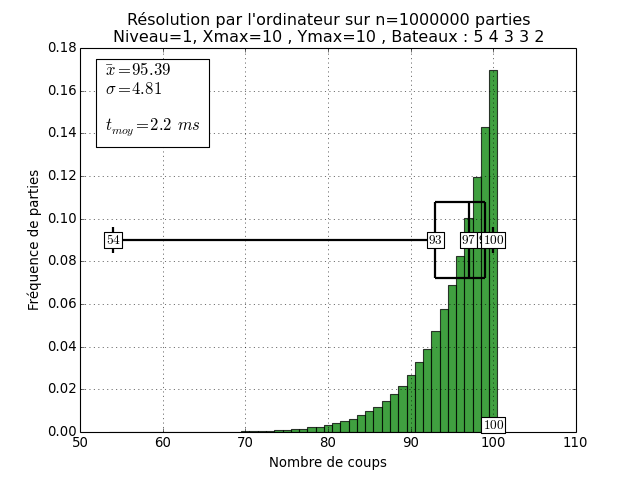
\includegraphics[scale=0.4]{./media/distrib_HAL_niveau=1_n=1000000.png}}
\end{center}
\end{frame}

\begin{frame}{Niveau 2}
Résultats sur $n=1\,000\,000$ parties :
\begin{center}
\fbox{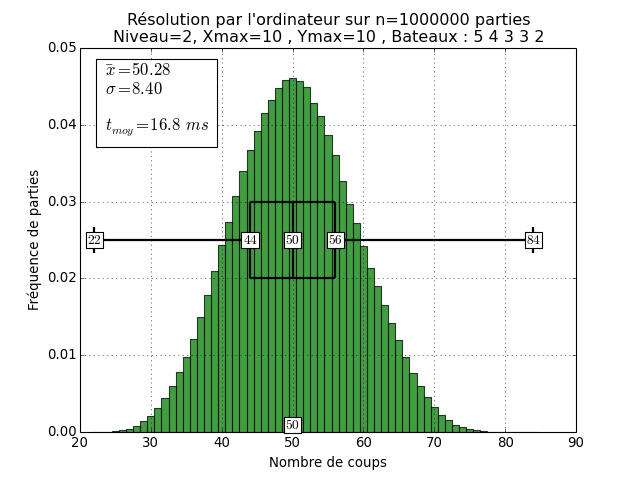
\includegraphics[scale=0.4]{./media/distrib_HAL_niveau=2_n=1000000.png}}
\end{center}
\end{frame}

\begin{frame}{Niveau 3}
Résultats sur $n=1\,000\,000$ parties :
\begin{center}
\fbox{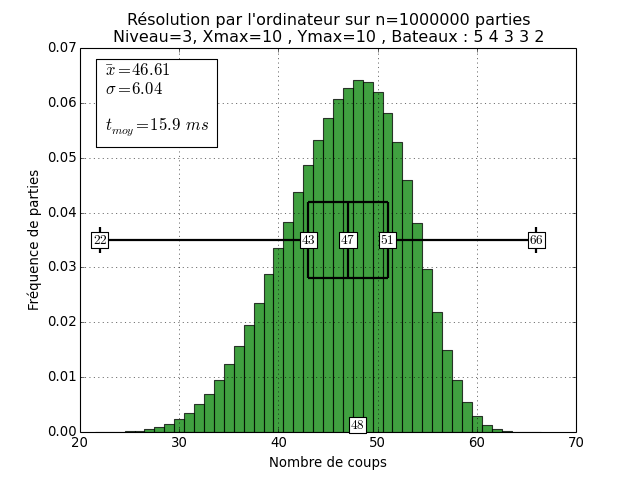
\includegraphics[scale=0.4]{./media/distrib_HAL_niveau=3_n=1000000.png}}
\end{center}
\end{frame}


\begin{frame}{Niveau 4(10)}
Résultats sur $n=100\,000$ parties :
\begin{center}
\fbox{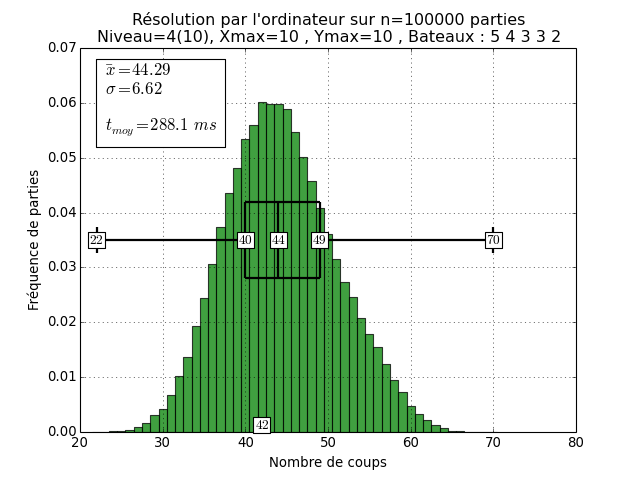
\includegraphics[scale=0.4]{./media/distrib_HAL_niveau=4(10)_n=100000.png}}
\end{center}
\end{frame}

\begin{frame}{Niveau 4(100)}
Résultats sur $n=10\,000$ parties :
\begin{center}
\fbox{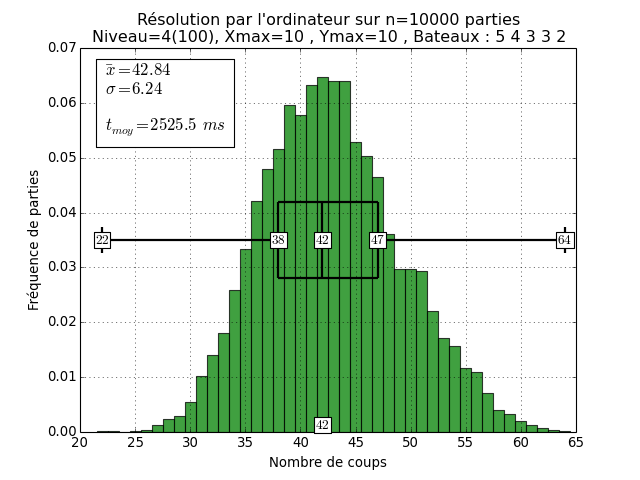
\includegraphics[scale=0.4]{./media/distrib_HAL_niveau=4(100)_n=10000.png}}
\end{center}
\end{frame}

\begin{frame}{Niveau 4(1000)}
Résultats sur $n=1\,000$ parties :
\begin{center}
\fbox{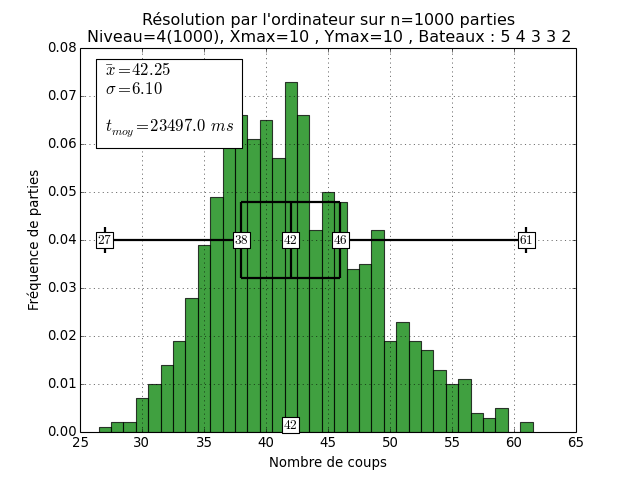
\includegraphics[scale=0.4]{./media/distrib_HAL_niveau=4(1000)_n=1000.png}}
\end{center}
\end{frame}

\begin{frame}{Niveau 4(10000)}
Résultats sur $n=100$ parties :
\begin{center}
\fbox{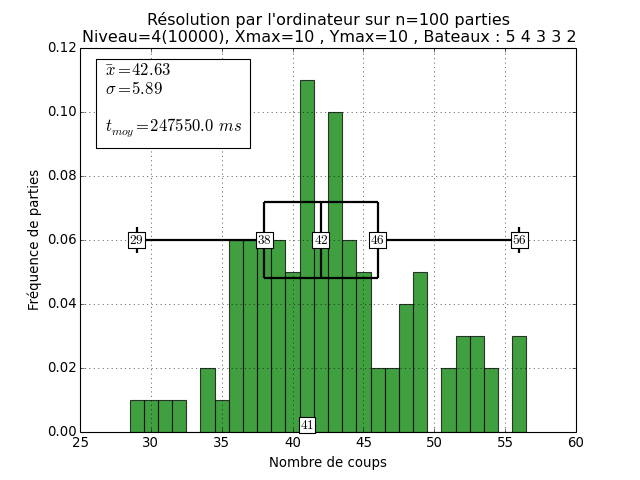
\includegraphics[scale=0.4]{./media/distrib_HAL_niveau=4(10000)_n=100.png}}
\end{center}
\end{frame}

\begin{frame}{Conclusion niveau 4}
\begin{center}
\begin{tabular}{|l|c|c|c|c|}
\hline
\no & 1 & 2 & 3 & 4\\
\hline
\texttt{nb\_echantillons} & 10 & 100 &  1\,000 & 10\,000\\
\hline
$n$ & 100\,000 & 10\,000 & 1\,000 & 100\\
\hline
$\conj x$ & 44,29 & 42,84 & 42,25 & 42,63\\
\hline
$\sigma$ & 6,62 & 6,24 & 6,10 & 5,89\\
\hline
$t_{moy}$ (en secondes)& 0,29 & 2,5 & 23,5 & 247\\
\hline 
\end{tabular}
\end{center}
\end{frame}

\begin{frame}
\begin{center}
\begin{tabular}{|l|l|c|}
\hline
\no & \texttt{nb\_echantillons} & Intervalle de confiance de $\mu$ \\
\hline
1 & 10 & $[44,25~;~44,33]$\\
\hline
2 & 100 & $[42,72 ~;~42,96]$\\
\hline
3 & 1\,000 & $[41,87~;~42,63]$\\
\hline
4 & 10\,000& $[41,48~;~43,78]$\\
\hline
\end{tabular}
\end{center}
\end{frame}


\begin{frame}{Niveau 5}
Résultats sur $n=1\,000\,000$ parties :
\begin{center}
\fbox{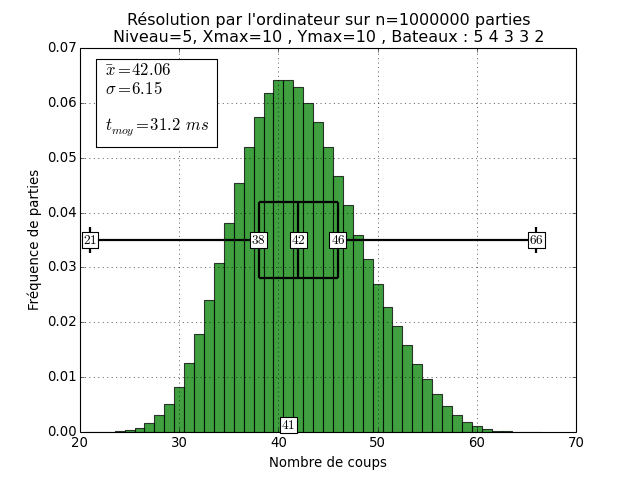
\includegraphics[scale=0.4]{./media/distrib_HAL_niveau=5_n=1000000.png}}
\end{center}
\end{frame}

\begin{frame}{Niveau 6(60)}
Résultats sur $n=10\,000$ parties :
\begin{center}
\fbox{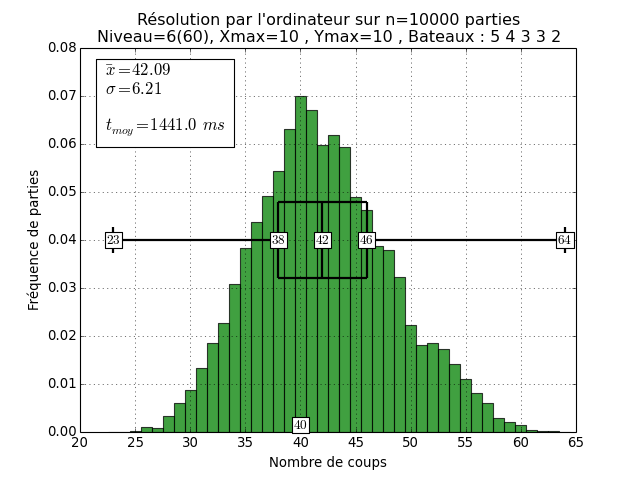
\includegraphics[scale=0.4]{./media/distrib_HAL_niveau=6(60)_n=10000.png}}
\end{center}
\end{frame}

\begin{frame}{Niveau 6(70)}
Résultats sur $n=1\,000$ parties :
\begin{center}
\fbox{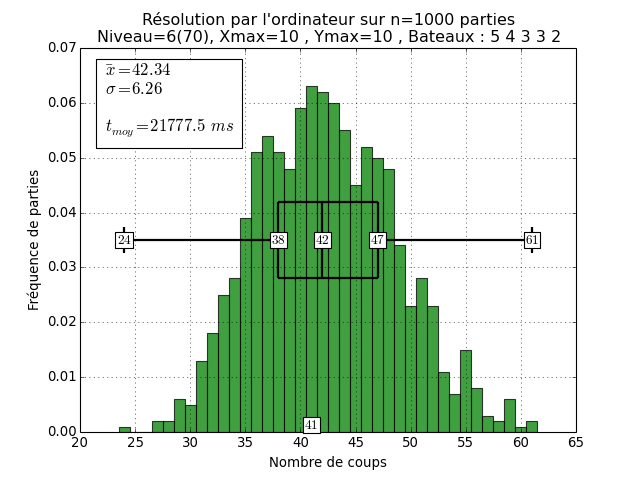
\includegraphics[scale=0.4]{./media/distrib_HAL_niveau=6(70)_n=1000.png}}
\end{center}
\end{frame}

\begin{frame}{Conclusion niveau 6}
\begin{center}
\begin{tabular}{|l|l|c|c|c|c|}
\hline
\no & Niveau & $n$ &  $\conj x$ & $\sigma$ & Intervalle de confiance\\
\hline
1 & 5 & 1\,000\,000 & 42,06 & 6,15 & $[42,05~;~42,07]$ \\
\hline
2 & 6(60) & 10\,000 & 42,09 & 6,21 & $[41,97~;~42,21]$\\
\hline
3 & 6(70) & 1\,000 & 42,34 & 6,26 & $[41,95~;~42,73]$\\
\hline
\end{tabular}
\end{center}
\end{frame}



\end{document}